\section{Verschiedene Transformationen}
\begin{minipage}{13.5cm}
\subsection{Berechnung}
\tiny
\begin{tabular}{|l|l|l|}
\hline
  \textbf{Transformation}
  & \textbf{Vorwärts}
  & \textbf{Rückwärts} \\
\hline
  Fourier-Reihe
  & $c_k=\frac{1}{T}\int_0^T{f(t) e^{-jk\omega_1 t}dt}$
  & $f(t) = \sum\limits_{k = -\infty}^{\infty} c_k  e^{j k \omega_1 t}$ \\
\hline
  Fourier-Integral
  & $F(\omega) = \int\limits_{-\infty}^{\infty} f(t)e^{-j\omega t}dt$
  & $f(t) =  \frac{1}{2\pi}\int\limits_{-\infty}^{\infty}
    F(\omega)e^{j\omega t}d\omega$ \\
\hline
  Laplace-Transformation
  & $F(s)=\int\limits_0^\infty f(t)e^{-st}dt$
  & Polynomdivision $\Rightarrow$ Partialbruchzerlegung $\Rightarrow$ Tabelle!\\
\hline
  Diskrete Fouriertransformation
  & $F(k) = \sum\limits_{n=0}^{N-1} f(n) e^{-j 2 \pi \frac{n}{N} k}$
  & $f^*(k) = \frac{1}{N} DFT(F^* (k))$\\
\hline
  Z-Transformation ($z = e^{j s T}$)
  & $F(z) = \sum\limits_{n=0}^{\infty} f(n) z^{-n}$
  & Polynomdivision $\Rightarrow$ Partialbruchzerlegung $\Rightarrow$ Tabelle!\\
\hline
\end{tabular}
\normalsize
\end{minipage}
\begin{minipage}{5.5cm}
\subsection{Pol/Nullstellentransfo}
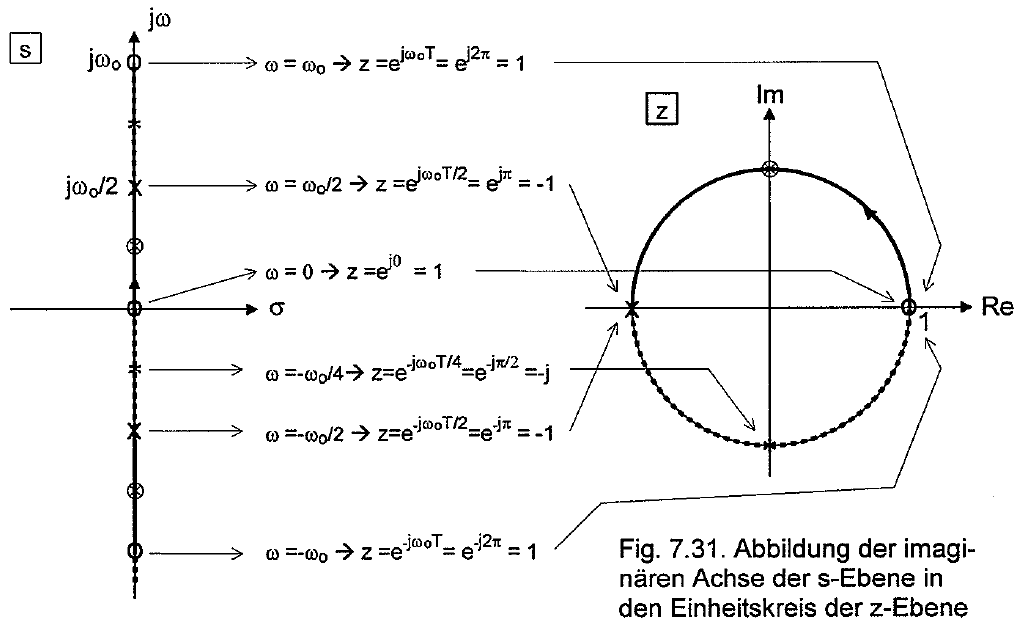
\includegraphics[width=5.5cm]{bilder/ImagAchse-Einheitskreis.png}
\end{minipage}

\section{Eigenschaften von Fourier- und Z-Transformation}
\tiny
\renewcommand{\arraystretch}{1.1}
\begin{tabular}{|p{3.2cm}||p{1.5cm}|p{1.8cm}||p{2.5cm}|p{2.5cm}||p{1.7cm}|p{3cm}|}
\hline
\textbf{Bezeichnung}
  & \multicolumn{2}{|c||}{\textbf{Zeitbereich}}
  & \multicolumn{2}{|c||}{\textbf{Kontinuierlicher Frequenzbereich}}
  & \multicolumn{2}{|c|}{\textbf{Diskreter Frequenzbereich}} \\
  & \textbf{kontinuierlich}
  & \textbf{diskret}
  & \textbf{Fourier-Integral}
  & \textbf{Laplace}
  & \textbf{Diskrete FT}
  & \textbf{Z-Transformation} \\
\hline
\hline
  Linearität
  & $\alpha\cdot f(t) + \beta\cdot g(t)$
  & $\alpha\cdot f(n) + \beta\cdot g(n)$
  & $\alpha\cdot F(\omega) + \beta\cdot G(\omega)$
  & $\alpha\cdot F(s) + \beta\cdot G(s)$
  & $\alpha\cdot F(n) + \beta\cdot G(n)$
  & $\alpha\cdot F(z) + \beta\cdot G(z)$\\
\hline
  "Ahnlichkeit / Zeitskalierung bzw. Spiegelung an Y-Achse
  &	$f(\alpha t)$
  & $f(-n)$
  & $\frac{1}{|\alpha|}F \left (\frac{\omega}{\alpha} \right)$
  & $\frac{1}{\alpha}F \left (\frac{s}{\alpha} \right )$
  & $F(-n)$
  & $F(z^{-1})$\\
\hline
  Dämpfung
  & -
  & $e^{dn} f(n)$
  & -
  & -
  & -
  & $F(z e^{d})$ \\
\hline
  Verschiebung im Zeitbereich
  & $f(t\pm t_0)$
  & $f(n \pm n_0)$
  & $e^{\pm j\omega t_0} F(\omega)$
  & $F(s)e^{\pm t_0 s}$
  & $e^{\pm j\frac{n}{N}2 \pi n_0} F(n)$
  & $z^{\pm n_0} F(z)$\\
\hline
  Verschiebung im Frequenzbereich
  & $f(t)e^{\mp\alpha t}$
  & $f(n) e^{\mp j \frac{n}{N} 2 \pi n_0}$
  & $F(\omega\pm \alpha)$
  & $F(s\pm\alpha)$
  & $F(n \pm n_0)$
  & $F(z \pm n_0)$\\
\hline
  Faltung im Zeitbereich
  &	$f(t) \ast g(t)$
  & $f(n) \ast g(n)$
  & $F(\omega) \cdot G(\omega)$
  & $F(s) \cdot G(s)$
  & $F(n) \cdot G(n)$
  & $F(z) \cdot G(z)$ \\
\hline
  Faltung im Frequenzbereich
  &	$f(t) \cdot g(t)$
  & $f(n) \cdot g(n)$
  & $\frac{1}{2\pi} F(\omega) \ast G(\omega)$
  & $\frac{1}{2\pi} F(s) \ast G(s)$
  & $\frac{1}{N} F(n) \ast G(n)$
  & $\frac{1}{N} F(z) \ast G(z)$\\
\hline
  Ableitungen im Zeitbereich bzw. Differenzenbildung
  & $\frac{\partial^n f(t)}{\partial t^n}$
  & $\Delta^k f(n)$
  & $(j\omega)^n F(\omega)$
  & $s^nF(s)-s^{n-1}f(0+)-s^{n-2}\frac{\partial f(0+)}{\partial t}-\ldots
 			-s^0\frac{\partial^{n-1} f(0+)}{\partial t^{n-1}}$
  &
  & $(1-z^{-1})^k F(z)$ \\
\hline
  Ableitung im Frequenzbereich
  & $(-t)^k\cdot f(t)$
  & $n f(n)$
  & $j^k \frac{-\partial^k F(\omega)}{\partial \omega^k}$
  & $\frac{\partial^k F(s)}{\partial s^k}$
  &
  & $-z \frac{\partial F(z)}{\partial z}$ \\
\hline
  Integration bzw. Summierung
  & $\int\limits_{-\infty}^t f(\tau)d\tau$
  & $\sum\limits_{n=0}^{k} f(n)$
  & $\frac{F(\omega)}{j\omega}+F(0)\pi\delta(\omega)$
  & $\frac{F(s)}{s}$
  &
  & $\frac{1}{1-z^{-1}} F(z)$ \\
\hline
  Anfangswert (Impulse)
  & $\lim\limits_{t\rightarrow 0} f(t)$
  & $f(0)$
  &
  & $\lim\limits_{s\rightarrow \infty} sF(s)$
  &
  & $\lim\limits_{z \rightarrow \infty} F(z)$ \\
\hline
  Endwert (Impulse)
  &	$\lim\limits_{t\rightarrow \infty} f(t)$
  & $\lim\limits_{n\rightarrow \infty} f(n)$
  &
  & $\lim\limits_{s\rightarrow 0} sF(s)$
  &
  & $\lim\limits_{z \rightarrow 1} ((1-z^{-1}) F(z))$\\
\hline
  Stabilität
  & -
  & -
  & -
  & Pole in LHE
  &
  & Pole innerhalb Einheitskreis \\
\hline
  Kausalität
  & -
  & -
  & A- \& Kausal
  & Nur Kausal
  &
  & $\lim\limits_{z \rightarrow \infty} z^{-1} F(z) = 0$ \\
\hline
\hline
  Spezial
  & \multicolumn{3}{l||}{
      Bessel-Theorem \qquad
      $\int\limits_{-\infty}^{\infty}f(t)g^{\ast}(t)dt =
         \frac{1}{2\pi}
         \int\limits_{-\infty}^{\infty}F(\omega)G^{\ast}(\omega)d\omega$}
  & \multicolumn{3}{|l|}{
      Parseval-Theorem \qquad
      $W = \int\limits_{-\infty}^{\infty}|f(t)|^2 dt = \frac{1}{2\pi}
      \int\limits_{-\infty}^{\infty}|F(\omega)|^2 d\omega$
    }\\
\hline
\end{tabular}
\renewcommand{\arraystretch}{1}\\
\normalsize

\begin{minipage}{11cm}
	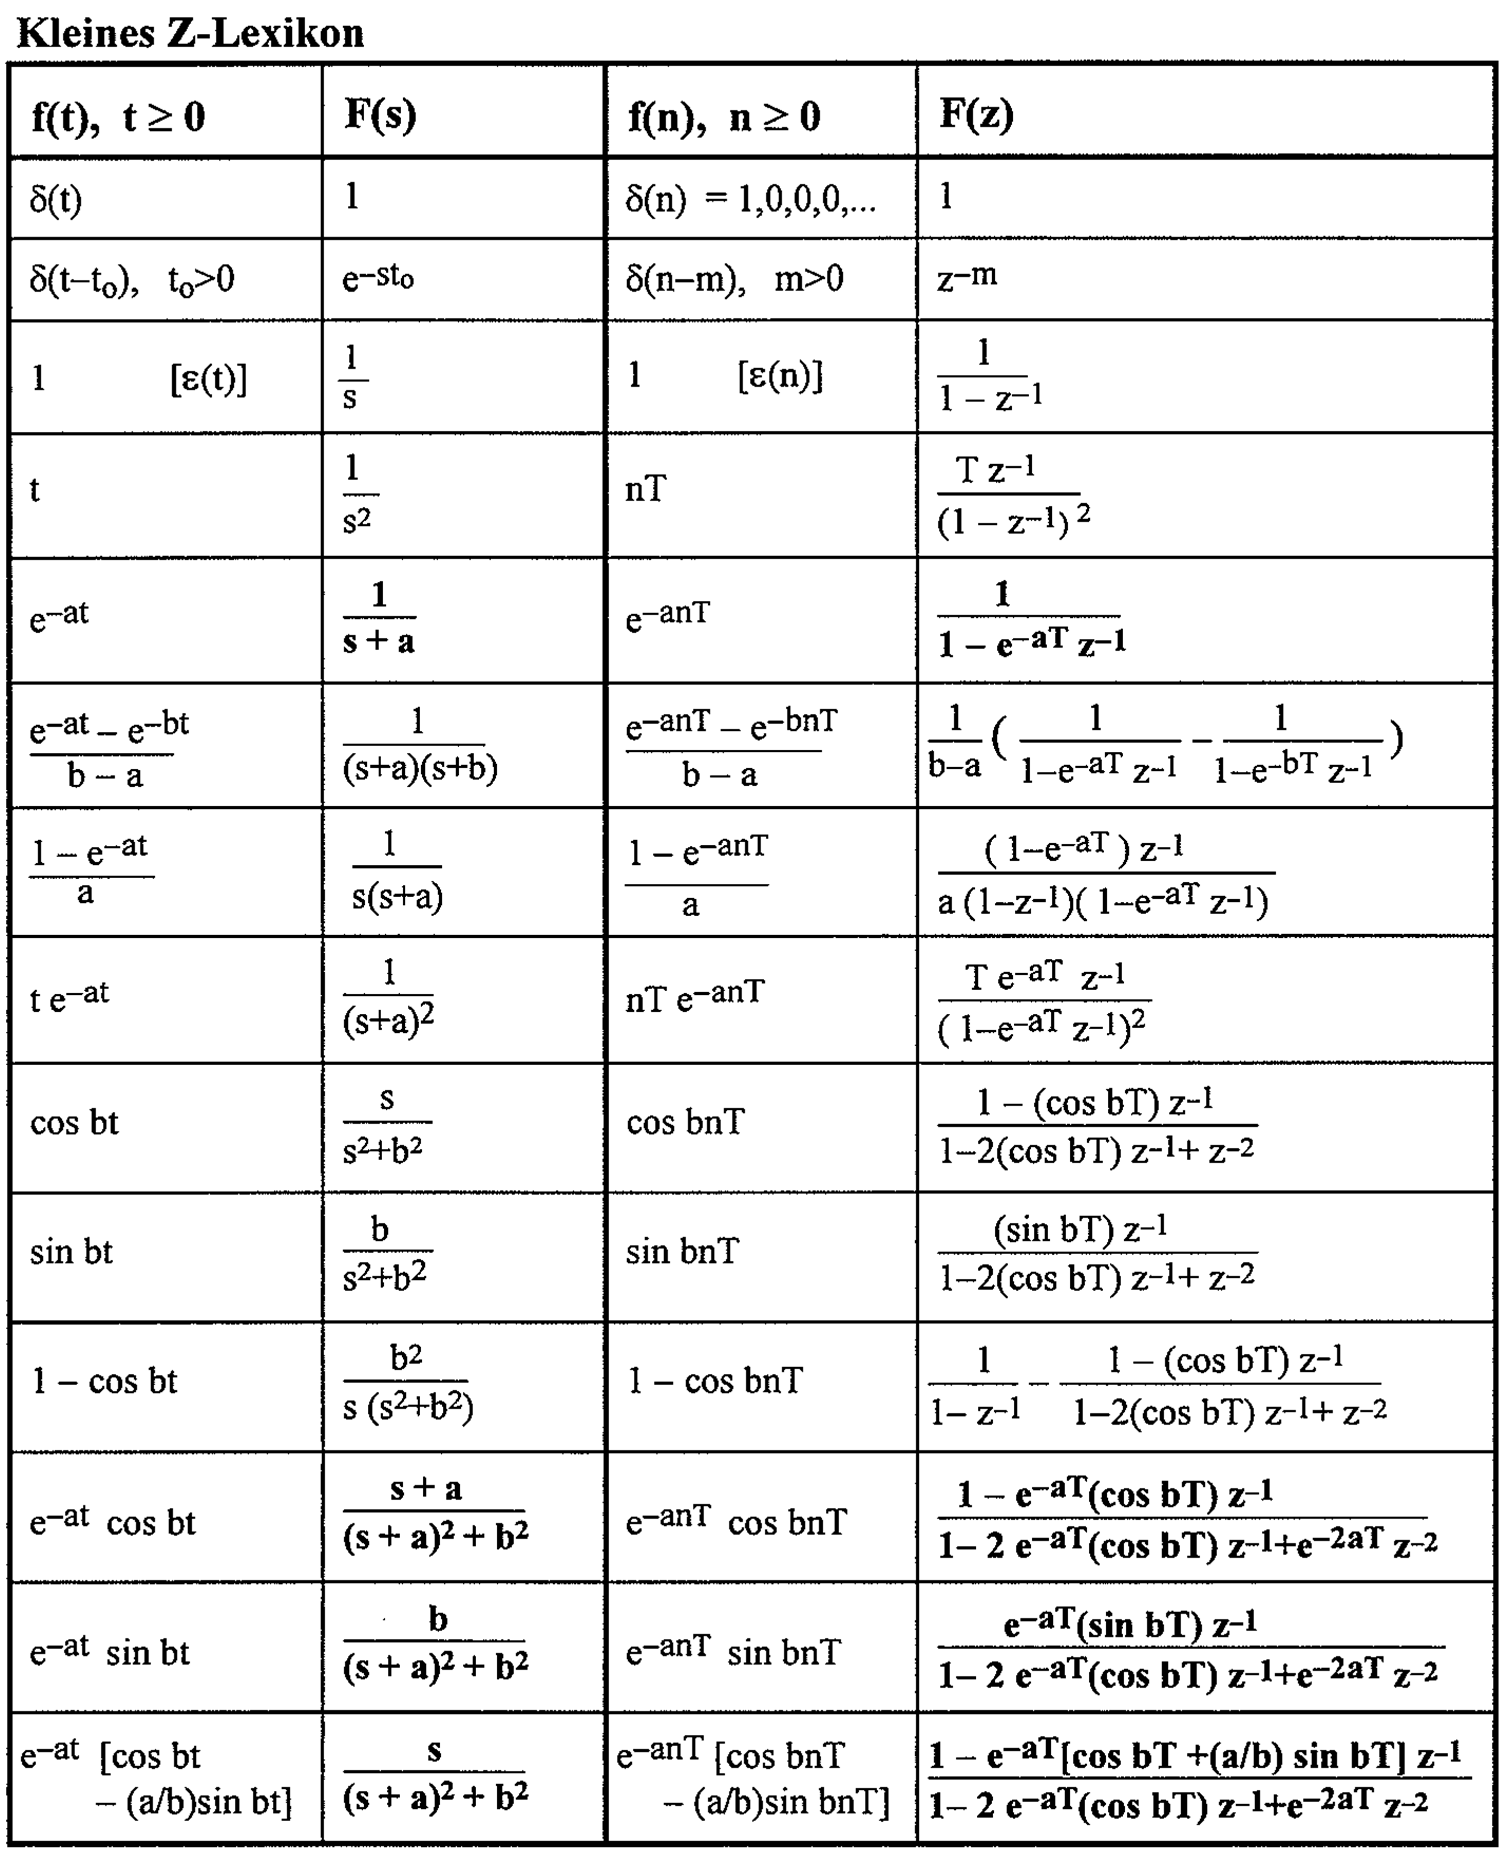
\includegraphics[height=11cm]{bilder/Z-Lexikon.png}
\end{minipage}
\begin{minipage}{8cm}
	$P_{ZOH}(z)=\frac{z-1}{z} Z_s \left\lbrace  \frac{P(s)}{s} \right\rbrace $\\
	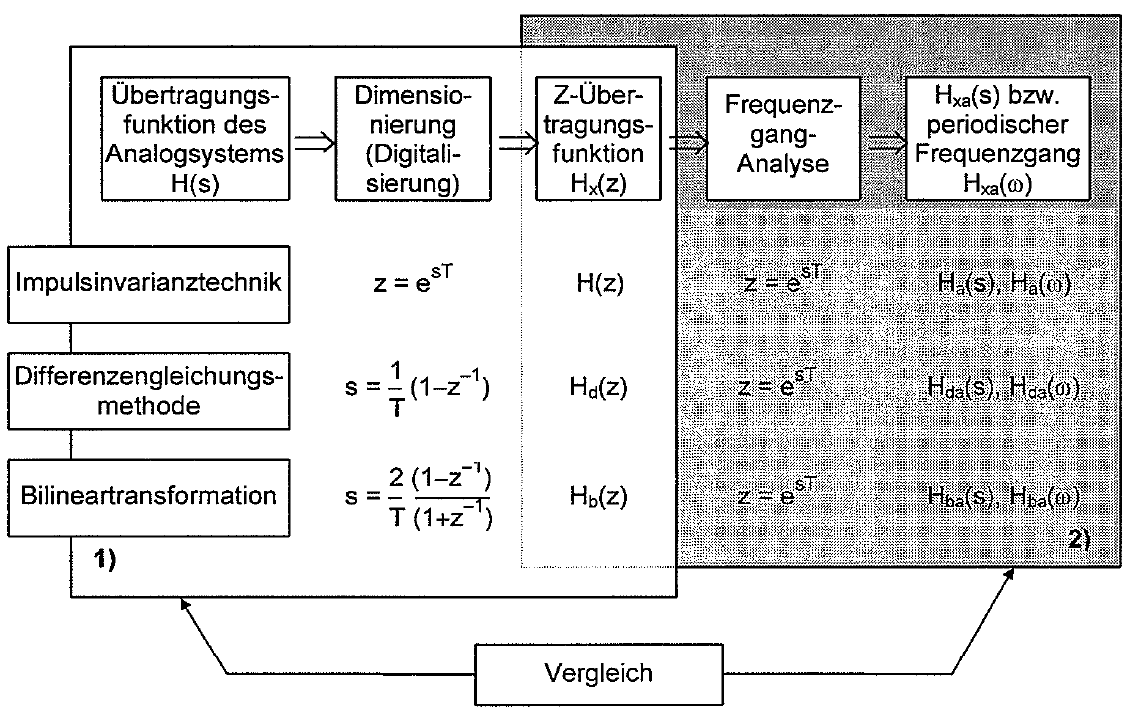
\includegraphics[width=8cm]{bilder/IIR-ArbeitsschritteundVarianten.png}
\end{minipage}
